% Created 2021-10-05 二 15:16
% Intended LaTeX compiler: xelatex
\documentclass[bigger]{beamer}
\usepackage{graphicx}
\usepackage{grffile}
\usepackage{longtable}
\usepackage{wrapfig}
\usepackage{rotating}
\usepackage[normalem]{ulem}
\usepackage{amsmath}
\usepackage{textcomp}
\usepackage{amssymb}
\usepackage{capt-of}
\usepackage{hyperref}
\usepackage{ctex}
\author{郑权}
\date{2021-06-05}
\title{某些类型链环投影图解纽数}
\hypersetup{
 pdfauthor={郑权},
 pdftitle={某些类型链环投影图解纽数},
 pdfkeywords={},
 pdfsubject={},
 pdfcreator={Emacs 28.0.50 (Org mode 9.5)}, 
 pdflang={English}}
\begin{document}

\maketitle
\tableofcontents

\section{研究背景}
\label{sec:org3491ef9}
\begin{enumerate}
\item 通俗地说,纽结理论就是要研究三维空间中的绳圈。
\label{sec:org3f69b41}
\begin{center}
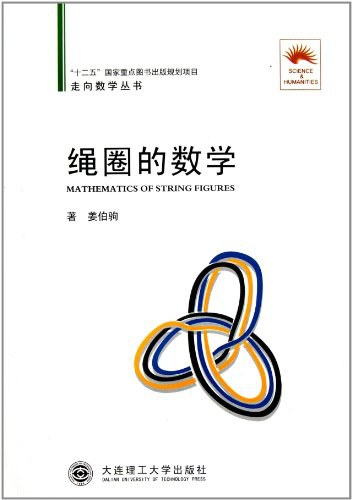
\includegraphics[width=.9\linewidth]{/home/vitalyr/projects/learn/Notebook/org/.attach/de/157e3c-139b-4fb5-9c86-cd7b376ebc6c/_20210411_145749screenshot.png}
\end{center}
\item 用数学的语言来说,纽结(knot)就是\(\mathbb{R}^{3}\) 中的简单闭曲线,链环(link)是\(\mathbb{R}^{3}\)中有限多条简单闭曲线的无交并
\label{sec:orga4d1cb6}
\begin{enumerate}
\item 构成链环的每一条简单闭曲线称为该链环的一个分支
\label{sec:org49567ee}
\item 可以把纽结看作只有一个分支的链环
\label{sec:org39474af}
\item 平面上的没有交叉点的简单闭曲线称为平凡纽结(unknot)
\label{sec:org5a513f4}
\end{enumerate}
\item 链环\(K\)用投影图来表示,投影图中的交叉点数记作\(c(K)\)
\label{sec:orga019cc1}
\begin{center}
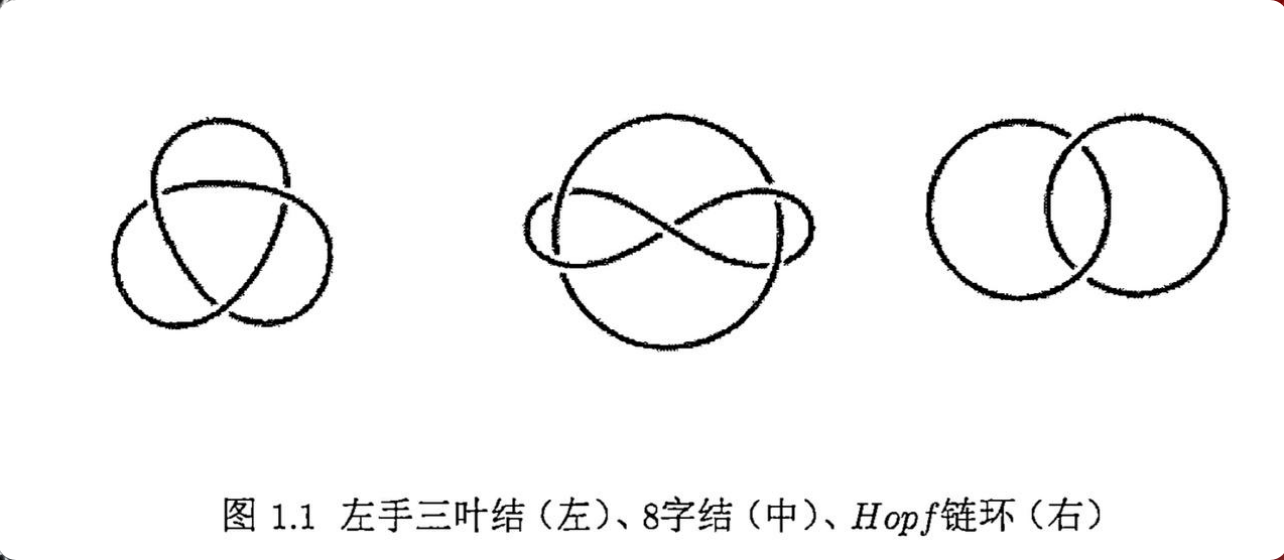
\includegraphics[width=.9\linewidth]{/home/vitalyr/projects/learn/Notebook/org/.attach/9e/0ba749-6979-40c8-943d-f4d86b9b56aa/_20210411_211308screenshot.png}
\end{center}
\item 纽结理论的中心问题是对纽结进行分类(up to homeomorphism)
\label{sec:org1e8753a}
\begin{center}
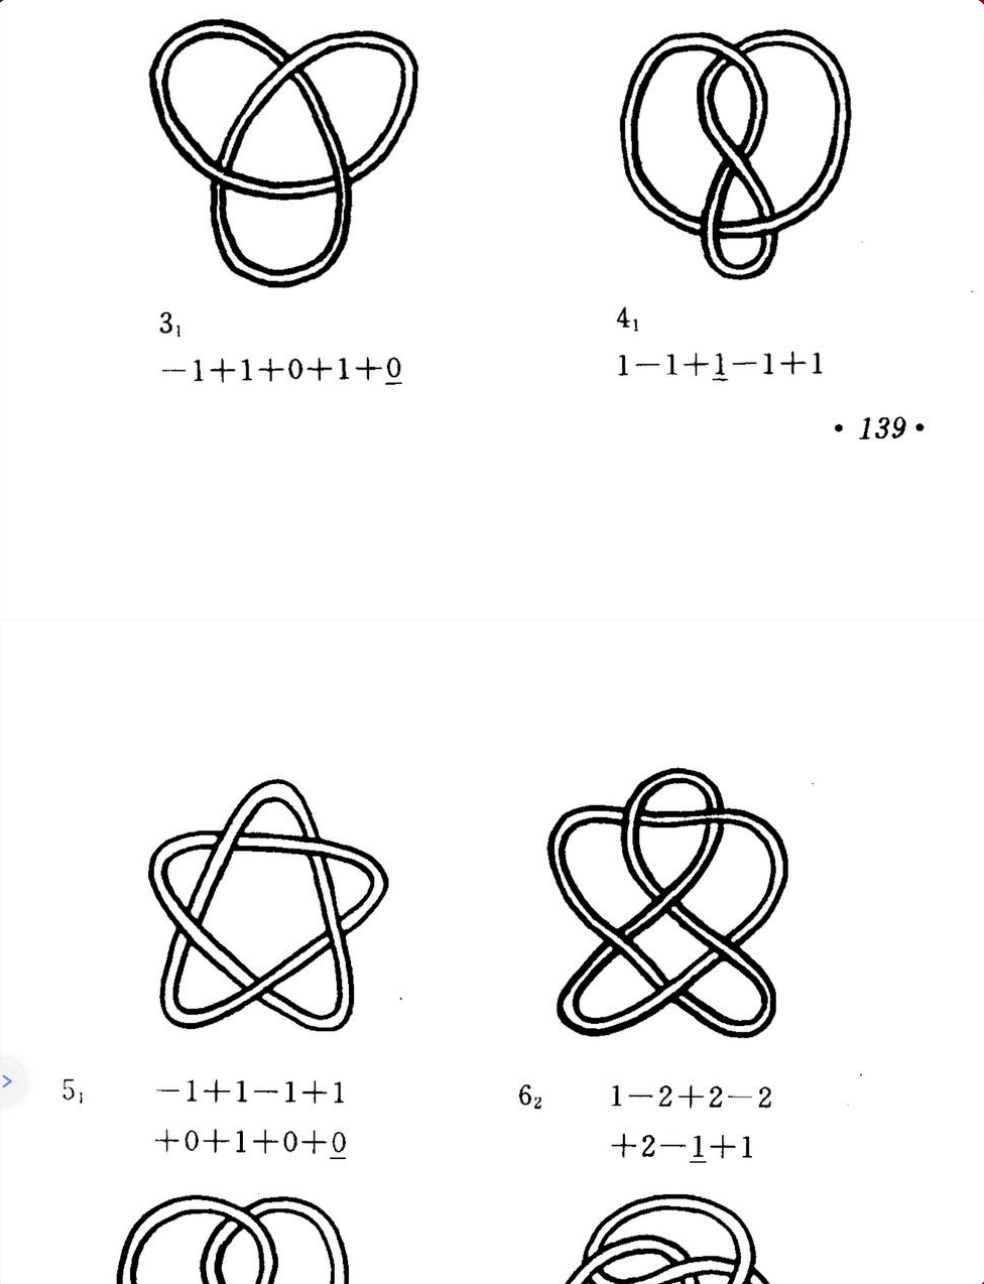
\includegraphics[width=.9\linewidth]{/home/vitalyr/projects/learn/Notebook/org/.attach/cf/4784d6-58d1-470f-b28e-8cda4a59f4c6/_20210411_205917screenshot.png}
\end{center}
\item 如何分类?使用各种纽结不变量
\label{sec:orgceee81b}
\begin{enumerate}
\item 交叉点数
\label{sec:org0e2d5d2}
\item bridge数
\label{sec:org7da4328}
\item 环绕数
\label{sec:orgd04c7ad}
\item 解纽数
\label{sec:org6d8a0c6}
\item 各种纽结多项式
\label{sec:org9aa9916}
\begin{enumerate}
\item 亚历山大多项式
\label{sec:org3feb0a4}
\item 琼斯多项式
\label{sec:org86a4256}
\item 括号多项式
\label{sec:org1965155}
\item HOMFLY多项式
\label{sec:org2da47d5}
\end{enumerate}
\item \ldots{}
\label{sec:orge2ba385}
\end{enumerate}
\item 研究意义
\label{sec:orgfa553d0}
\begin{enumerate}
\item 纽结应用在分子生物学上,有助于阐明DNA双螺旋结构、蛋白质的结构与功能等重大课题
\label{sec:org175ac08}
\item 量子混沌方面,1984年以来Birman等人应用纽结理论深入揭示了Lorenz吸引子的拓扑结构
\label{sec:org4f54aa4}
\item 2016年获得诺贝尔物理学奖的三位教授把拓扑和凝聚态物理结合起来,发现了物质的拓扑相变和拓扑相
\label{sec:orgfeeeee1}
\item \ldots{}
\label{sec:org9fda940}
\end{enumerate}
\end{enumerate}
\section{研究内容}
\label{sec:orgb5e4fe2}
\begin{enumerate}
\item 纽结或链环的解纽数(unknotting number)
\label{sec:org1a841b3}
\begin{enumerate}
\item 把一个链环\(K\)变换成平凡链环时所改变的交叉点的最小数,一般记作\(u(K)\)
\label{sec:orgbe95834}
\begin{center}
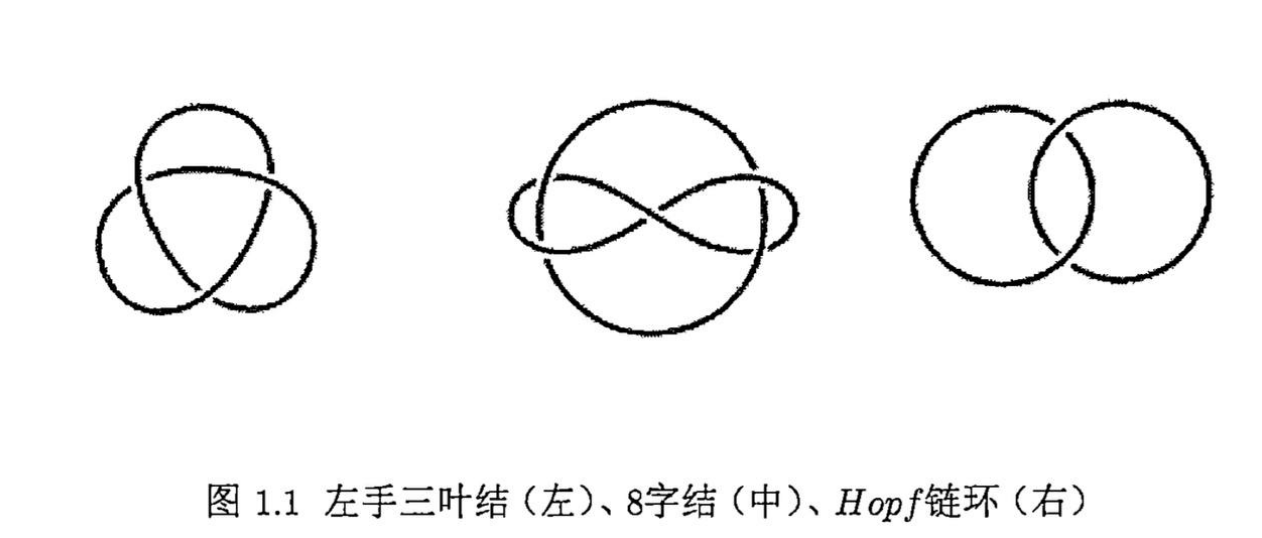
\includegraphics[width=.9\linewidth]{/home/vitalyr/projects/learn/Notebook/org/.attach/72/d84080-51b9-4c1c-824b-8a0910c6e6a6/_20210411_213150screenshot.png}
\end{center}

上图中,左手三叶结的解纽数是1,8字结的解纽数是2,Hopf链环的解纽数是1.
\end{enumerate}

\item 交错链环
\label{sec:orgad85ee7}
如果链环的“线”在一个交叉点在下,而在任何相邻的交叉点都在上,或者反过来,那就称它为交错链环(alternating link)。
下面左手三叶结是一个交错纽结:

\begin{center}
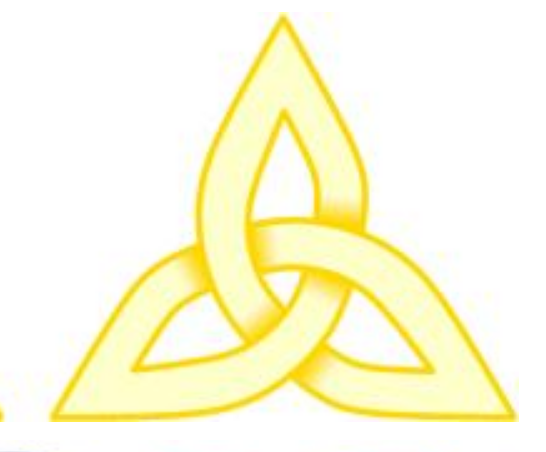
\includegraphics[width=.9\linewidth]{/home/vitalyr/projects/learn/Notebook/org/.attach/29/9f1f51-05f0-445a-a7cf-ec62a618f87f/_20210605_110121screenshot.png}
\end{center}

例如下面这个链环不是交错纽结:
\begin{center}
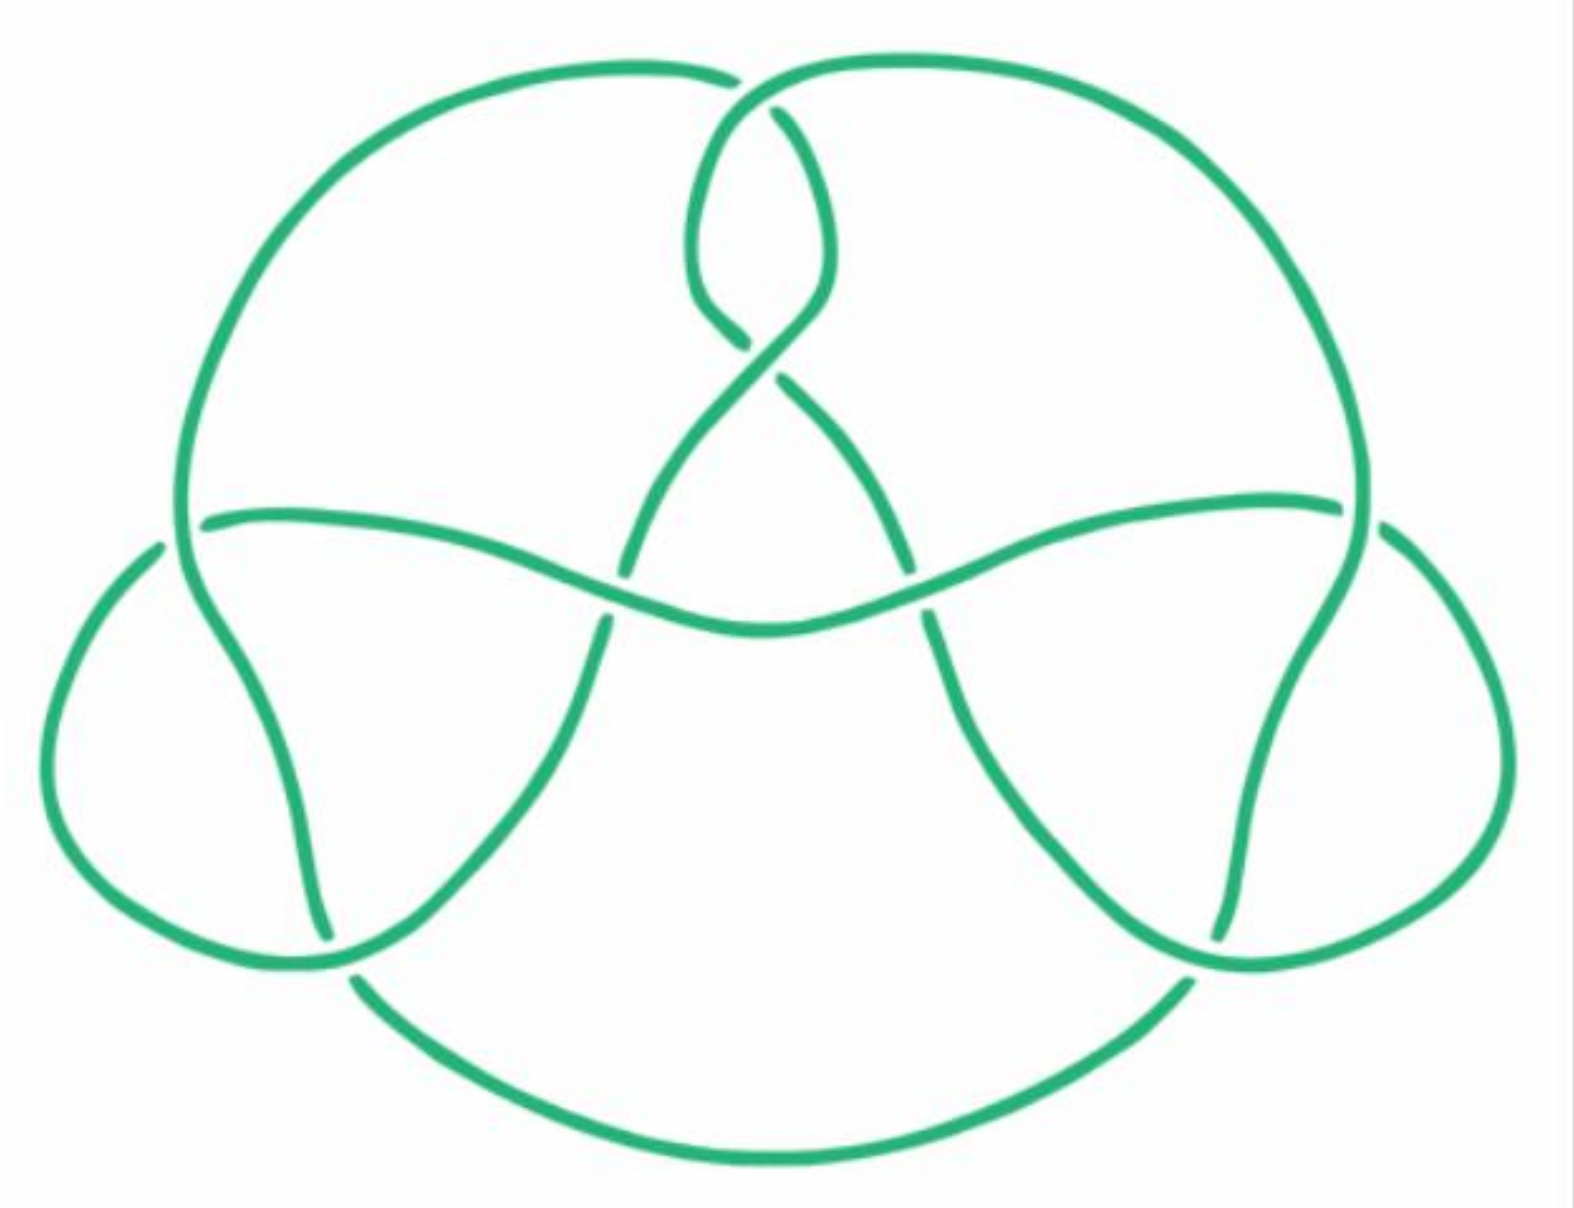
\includegraphics[width=.9\linewidth]{/home/vitalyr/projects/learn/Notebook/org/.attach/29/9f1f51-05f0-445a-a7cf-ec62a618f87f/_20210605_083014screenshot.png}
\end{center}
论文的结果依赖于交错链环是非平凡的这一性质
\item Kanenobu纽结
\label{sec:org8f31657}
由日本数学家Kanenobu在1986年在[9]中提出的一族具有相同琼斯多项式的纽结

\begin{center}
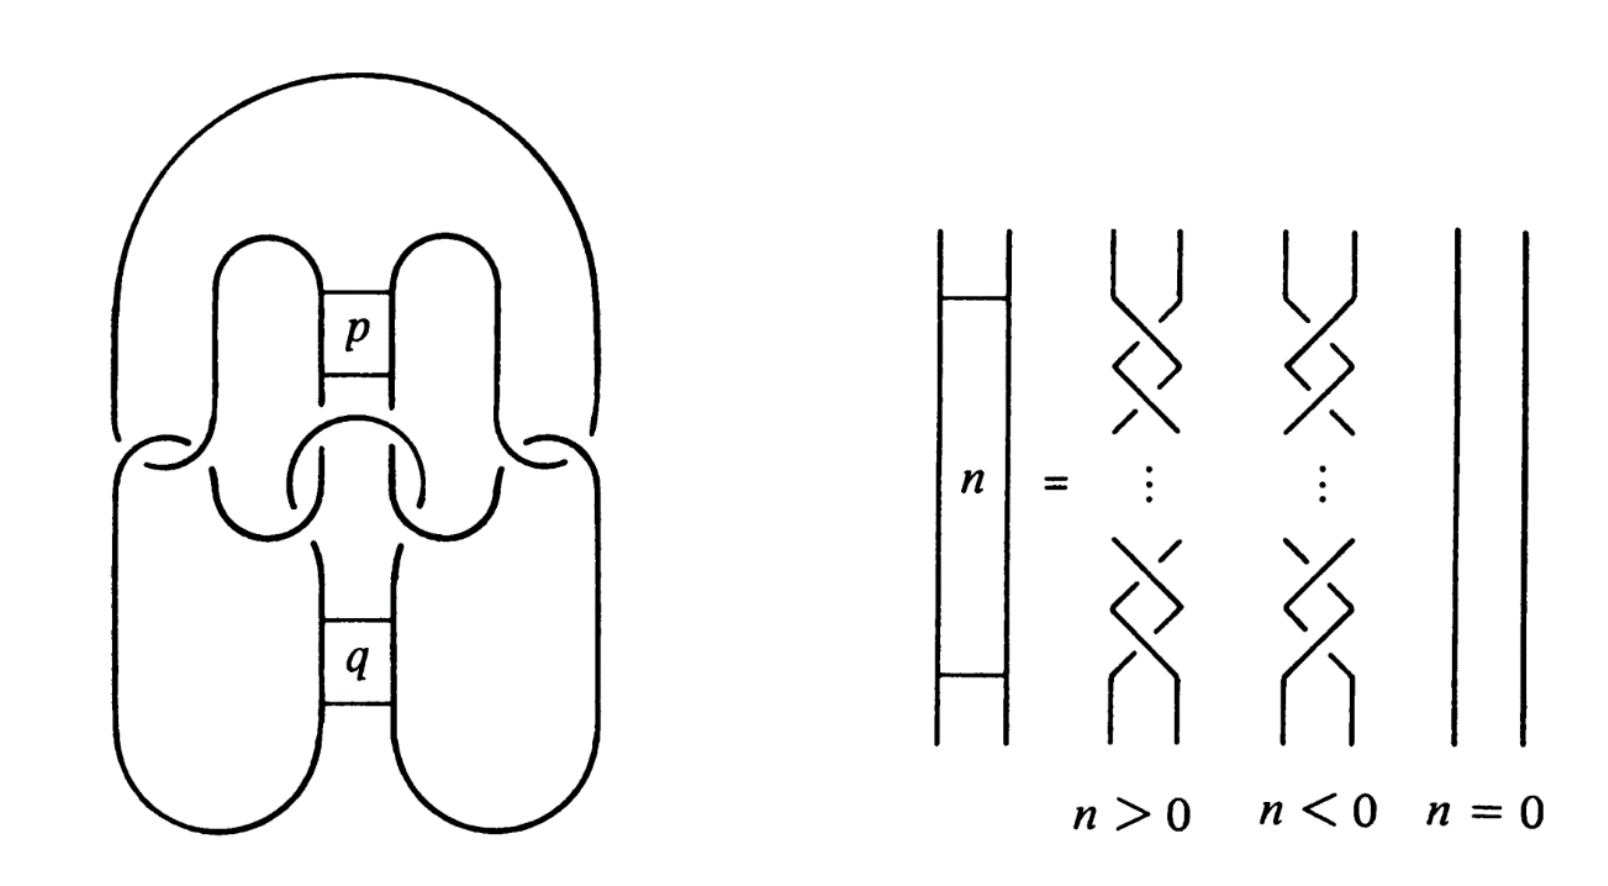
\includegraphics[width=.9\linewidth]{/home/vitalyr/projects/learn/Notebook/org/.attach/29/e7c797-3d58-4399-8938-08aed6aec0ec/_20210605_110029screenshot.png}
\end{center}
\end{enumerate}


\section{国内外研究现状}
\label{sec:org98edfdd}
\begin{enumerate}
\item 1991年S.Fukuhara、Y. Matsumoto、O. Saeki 给出了一些类型torus纽结的解纽数的证明 [1]
\label{sec:orgca3289d}
对于\((p,q)=(2,q),(3,4),(3,5),(3,7),(3,8),(3,10),(4,5)\),有
\(u(T(p,q))=\frac{(p-1)(q-1)}{2}\)
\item 2004年,Owens给出了所有交叉点小于等于9的纽结的解纽数.[3]
\label{sec:org9ccaec4}
\item 1984年,Beiler给出了一个奇妙的例子:对于一个纽结,它的极小投影图有10个交叉点,它不可能用少于三个交叉点的改变来变成平凡纽结,但它有个14个交叉点的投影图,与之同痕,但可以用两个交叉点的改变来变为平凡纽结
\label{sec:org91f78d9}
\item 2014年,V. Siwach, P. Madeti给出了多于700种交叉点数在10-16的torus纽结的解纽数.[4]
\label{sec:orgb1b4c9b}
\end{enumerate}
\section{研究成果}
\label{sec:org91037ab}
\begin{enumerate}
\item 求出Kanenobu纽结\(K(0, 0)\)的解纽数是2\hfill{}\textsc{ATTACH}
\label{sec:orge7b3698}
:ID:       cbef0049-b628-4f6d-8671-a3b10a2d8ce7
\begin{center}

\includegraphics[width=.9\linewidth]{/home/vitalyr/projects/learn/Notebook/org/.attach/3e/0d404b-0b10-45ad-8da1-9b6b25beacf6/_20210625_084436screenshot.png}
\end{center}
\item 求出了推广的Kanenobu纽结\(K(p, q, n)\)的解纽数是2,与\(p, q, n\)无关:\hfill{}\textsc{my\_org\_tag}
\label{sec:org3a62550}
\begin{enumerate}
\item 首先说明\(K(p, q, n)\)是非平凡的,这由参考文献[8]里的定理5保证:
\label{sec:org3b3a10b}
The Khovanov homology for generalized Kanenobu knot:
\(Kh(K_{\beta}(p,q)) \cong Kh(K_{\beta}(p+1, q-1))\)
\item 然后说明改变2号和9号交叉点可以可以使之成为平凡纽结
\label{sec:orgfafc264}
\end{enumerate}

\item 在进一步推广Kanenobu纽结\(K(p, q, m, n, l)\)非平凡的前提下,得到它的解纽数
\label{sec:orgc1354c9}
\begin{center}
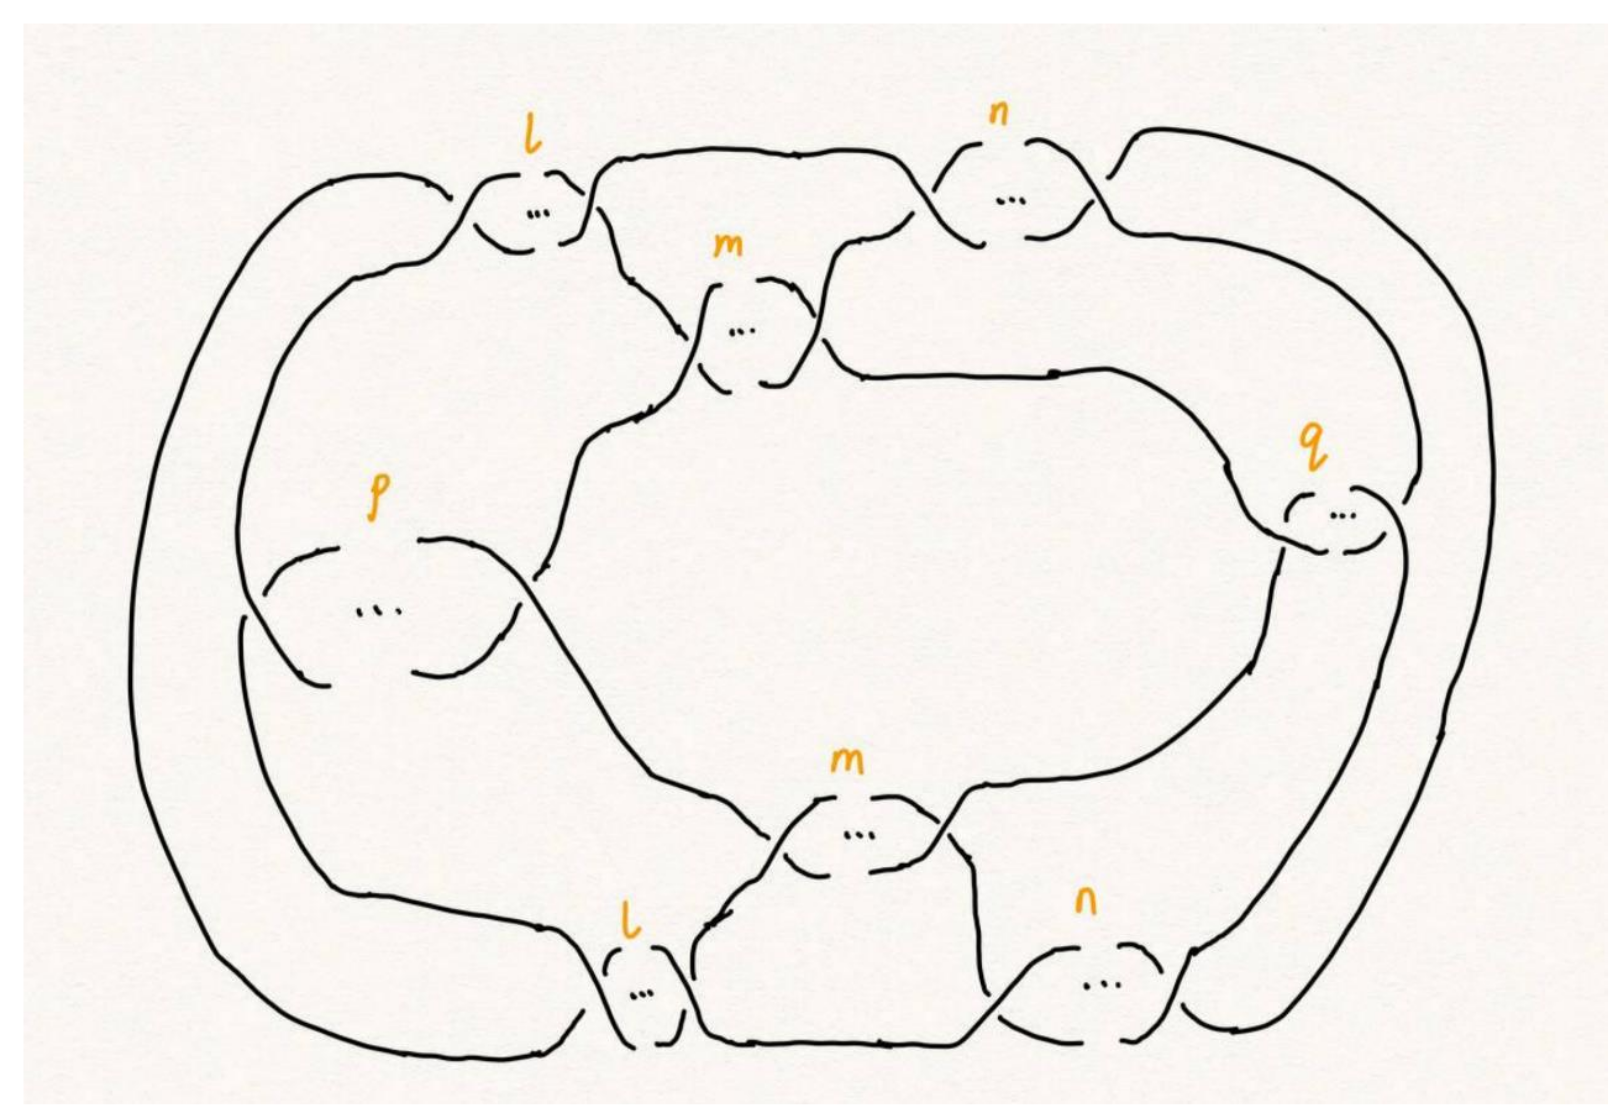
\includegraphics[width=.9\linewidth]{/home/vitalyr/projects/learn/Notebook/org/.attach/66/a09525-7b6b-41b8-b11a-fac7dcd37c33/_20210605_070844screenshot.png}
\end{center}

\begin{enumerate}
\item When \(m>n\), after changes the crossing points in the \(m\)and \(l\) part (do this by reducing \([\frac{m+l}{2}]\) crossing points), we get the knot like:
\label{sec:org30d6c5a}

\begin{center}
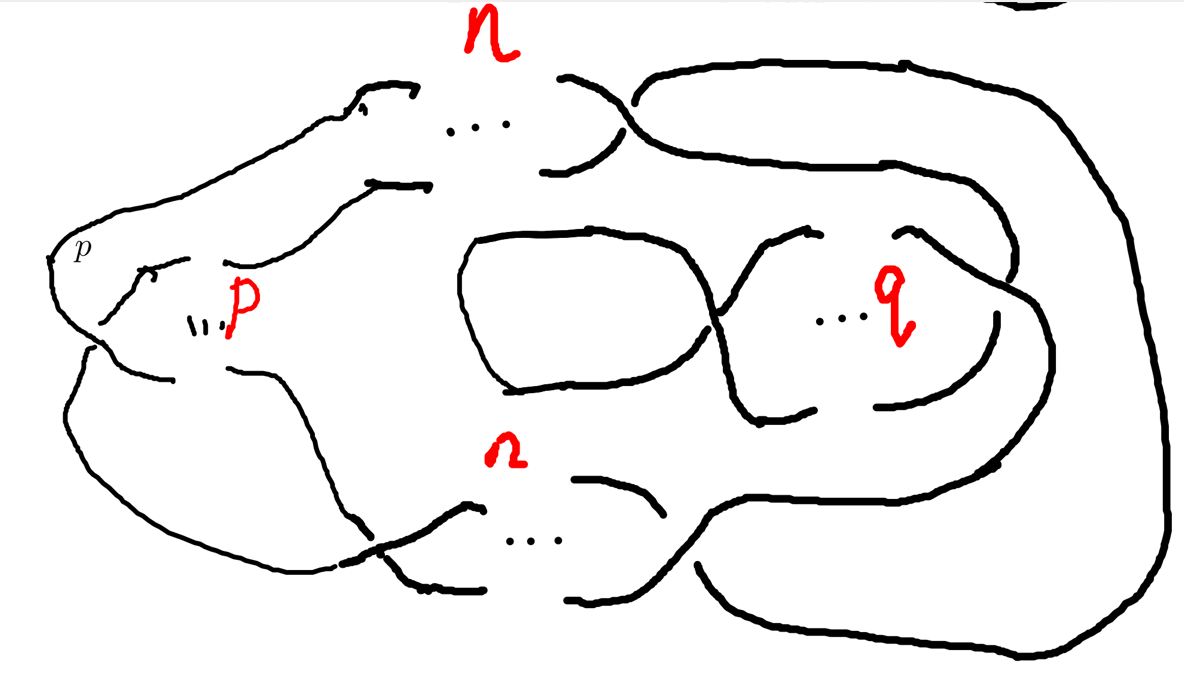
\includegraphics[width=.9\linewidth]{/home/vitalyr/projects/learn/Notebook/org/.attach/66/a09525-7b6b-41b8-b11a-fac7dcd37c33/_20210605_071429screenshot.png}
\end{center}
\item When \(n>m\), after changing the crossing points in \(n\) and \(l\) part(do this by reducing \([\frac{n+l}{2}]\) crossing numbers), we get the knot like:
\label{sec:org6df26ef}
\begin{center}
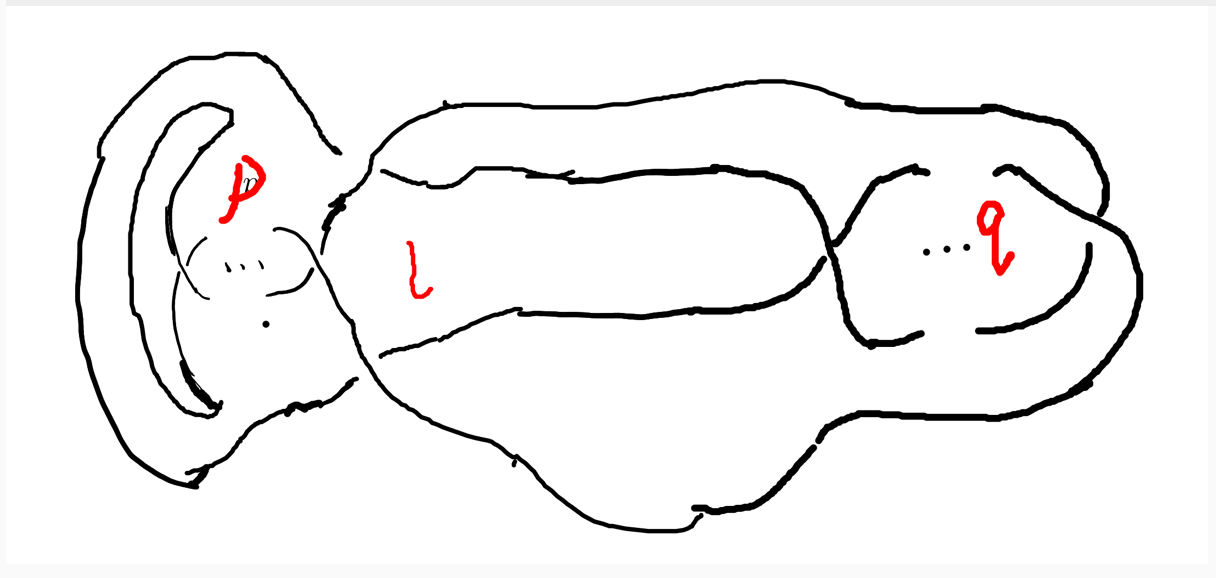
\includegraphics[width=.9\linewidth]{/home/vitalyr/projects/learn/Notebook/org/.attach/66/a09525-7b6b-41b8-b11a-fac7dcd37c33/_20210605_071532screenshot.png}
\end{center}
\item When \(q + n < m + l\) and \(q + n < n + l\), we would untie the \(q\) and \(n\) part with \(2[\frac{q+n}{2}]\) changes, and get this:
\label{sec:org05c7f0e}
\begin{center}
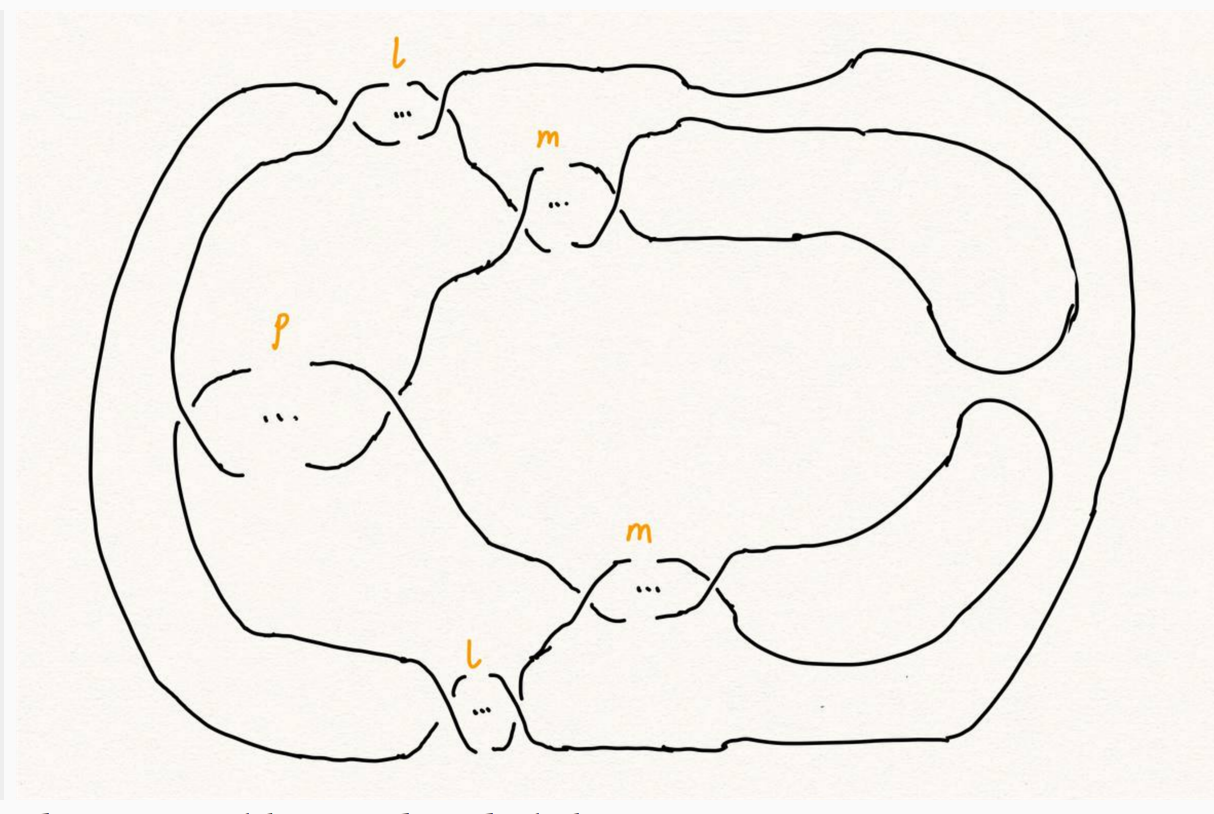
\includegraphics[width=.9\linewidth]{/home/vitalyr/projects/learn/Notebook/org/.attach/66/a09525-7b6b-41b8-b11a-fac7dcd37c33/_20210605_071607screenshot.png}
\end{center}
\end{enumerate}
\end{enumerate}
\section{总结}
\label{sec:org4a25204}
两次推广了Kanenobu纽结并给出它的解纽数,但最终的结果依赖于\(K(p, q, m, n, l)\)的非平凡性。

它的非平凡性直观上看比较显然,但若用琼斯多项式、\(\rm HOMFLY\)同调等工具来证明却非常麻烦,需要进一步研究。

一个两行两列的矩阵\(\frac{1}{2} \int\limits_{1}^{\infty}f(x)dx\)
\begin{equation}
\label{eq:1}
x ^{2} + y^{2} = z^{2}
\end{equation}
\begin{table}[htbp]
\caption[]{\label{tab:2} }
\vspace{4mm}
0 & 1 \\
1 & 0
\end{table}

\(f(x)\)
\section{参考资料}
\label{sec:org3aefbf4}
\begin{enumerate}
\item\relax [1] S.Fukuhara, Y.Matsumoto, O.Saeki, An estimate for the unknotting numbers of torus knots[J], Topology and its Applications, 1991, 38(3): 293-299
\label{sec:orgf029980}
\item\relax [2] 姜伯驹,绳圈的数学,湖南教育出版社[M],1991
\label{sec:org5eb5f93}
\item\relax [3] B. Owens, On slicing invariants of knots[J], Journal of Knot Theory and Its Ramifications, 2011, 14(01):3-8.
\label{sec:orgec3762f}
\item\relax [4] V.Siwach, P. Madeti, Unknotting Number of Some Knots[J], Elsevier, 2014
\label{sec:org2861f9b}
\item\relax [5] V. Siwach, M. Prabhakar, A Method for Unknotting Torus Knots[J], Mathematics, 2012
\label{sec:org662bd3a}
\item\relax [6] Rolfen, Knots and Links[M], Publish or Perish, 1976
\label{sec:org9401f1c}
\item\relax [7] W.B. Raymond Lickorish, Introduction to Knot Theory[M], Springer, 1997
\label{sec:org203d55d}
\item\relax [8] C.C. Adams, The Knot Book: An Elementary Introduction to the Mathematical Theory of Knots[M], W.H.Freeman and Company, New York, 1994
\label{sec:orgb77a548}
\item\relax [9] Kanenobu, T., Infinitely Many Knots with the Same Polynomial Invariant, Proceedings of the American Mathematical Society, 97(1), 158–162 (1986)
\label{sec:org4d1b44a}

感谢聆听,请老师批评指正!
\end{enumerate}
\end{document}
